\section{Appendix}
\subsection{Trainings Loop}\label{pcsam}
\begin{algorithm}
	\caption{SAM Training Algorithm}
	\begin{algorithmic}[1]
		\State Initialize ground truth mask $G$
		\State Initialize total number of iterations $n$
		\State Initialize logit mask $ P = \text{None}$
		\State Initialize threshold $t$
		\State Sample random integer $u\in \{k \in \mathbb{N}|k\leq n\}$
		\State Uniformly sample a foreground point $p$ from $G$
		\For{$i = 1$ to $n$}
		\State Predict new logit mask $P$ using point $p$ and logit mask $P$
		\If{i = u or i = n}
		\State \textbf{continue}
		\EndIf
		\State Update binarized mask $M_{\text{pred}} = P > t$ 
		\State Update error region $E = |G - M_{\text{pred}}|$
		\State Update point $p$ by sampling uniformly from error region $E$
		\If{$E(p)$ is false negative}
		\State $p$ is a foreground point
		\ElsIf{$E(p)$ is false positive}
		\State $p$ is a background point
		\EndIf
		\EndFor
	\end{algorithmic}
\end{algorithm}
\subsection{Losses and Learning Rate}\label{seclr}
\begin{figure}[H]
	\centering
	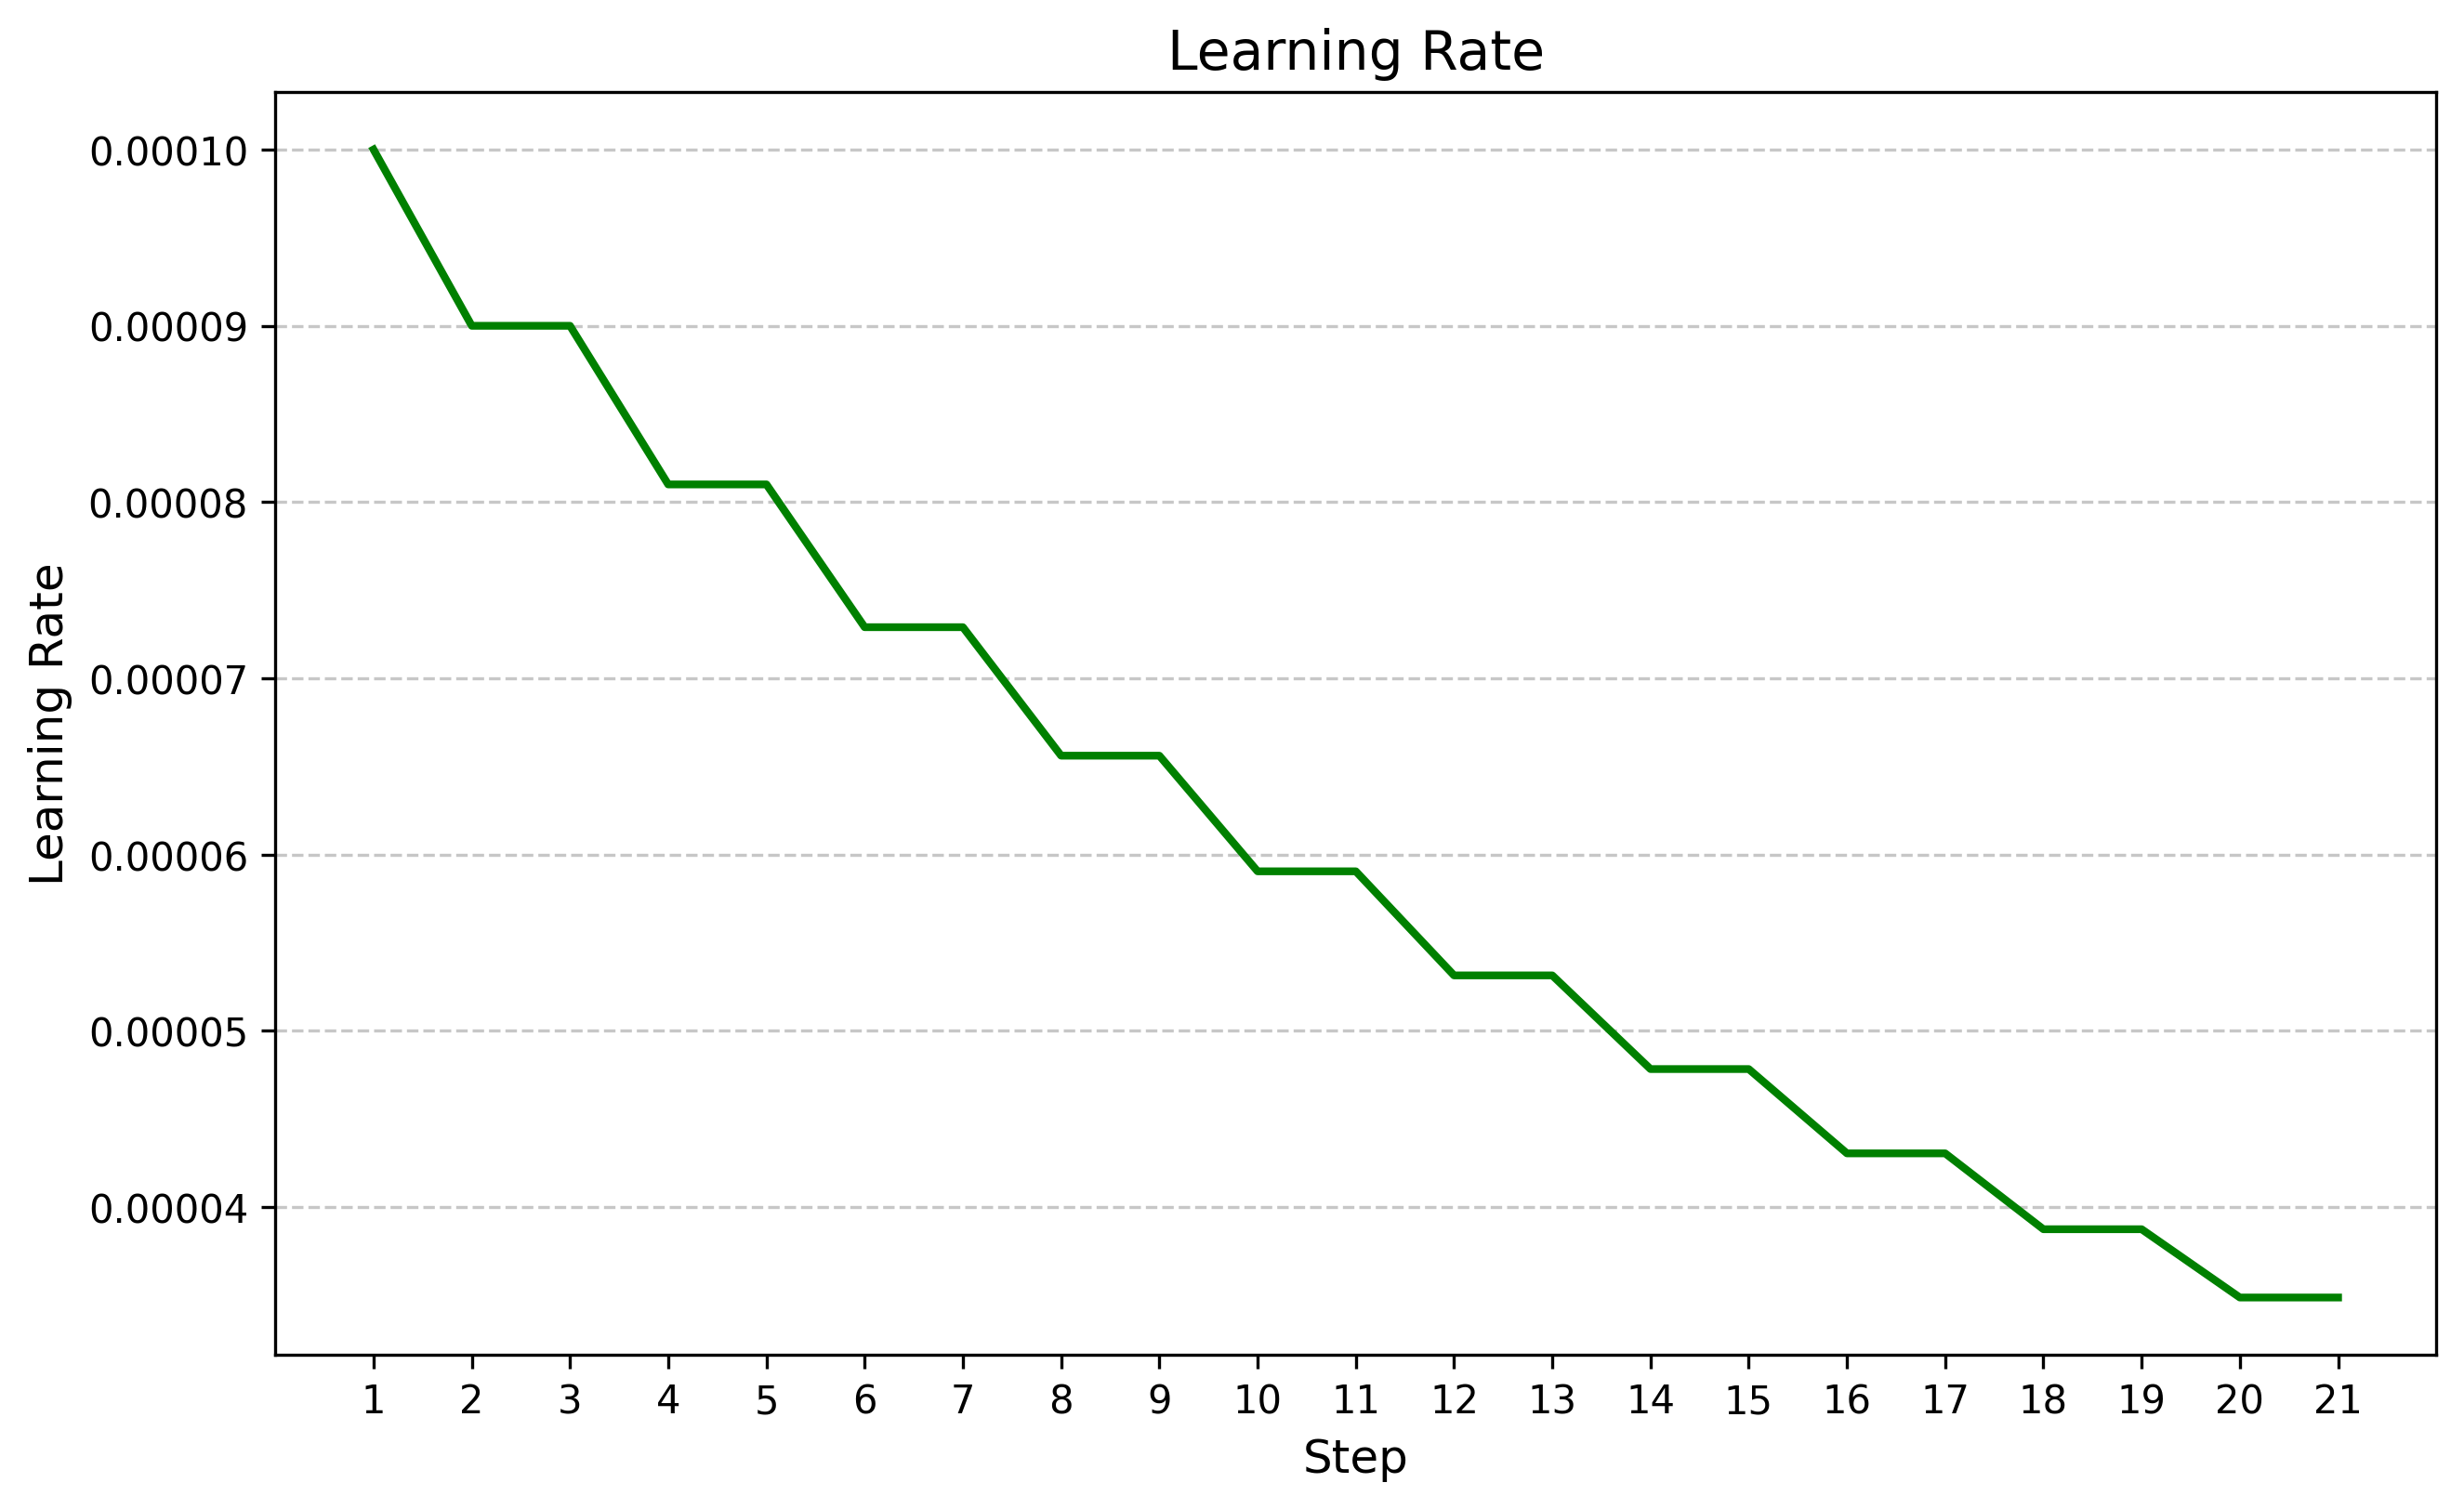
\includegraphics[width=\textwidth]{"images/lr.png"}
	\caption[Learning rate \texttt{MyoSAM}]{Progression of \texttt{MyoSAM} learning rate.}
	\label{figlr}
\end{figure}
\begin{figure}[H]
	\centering
	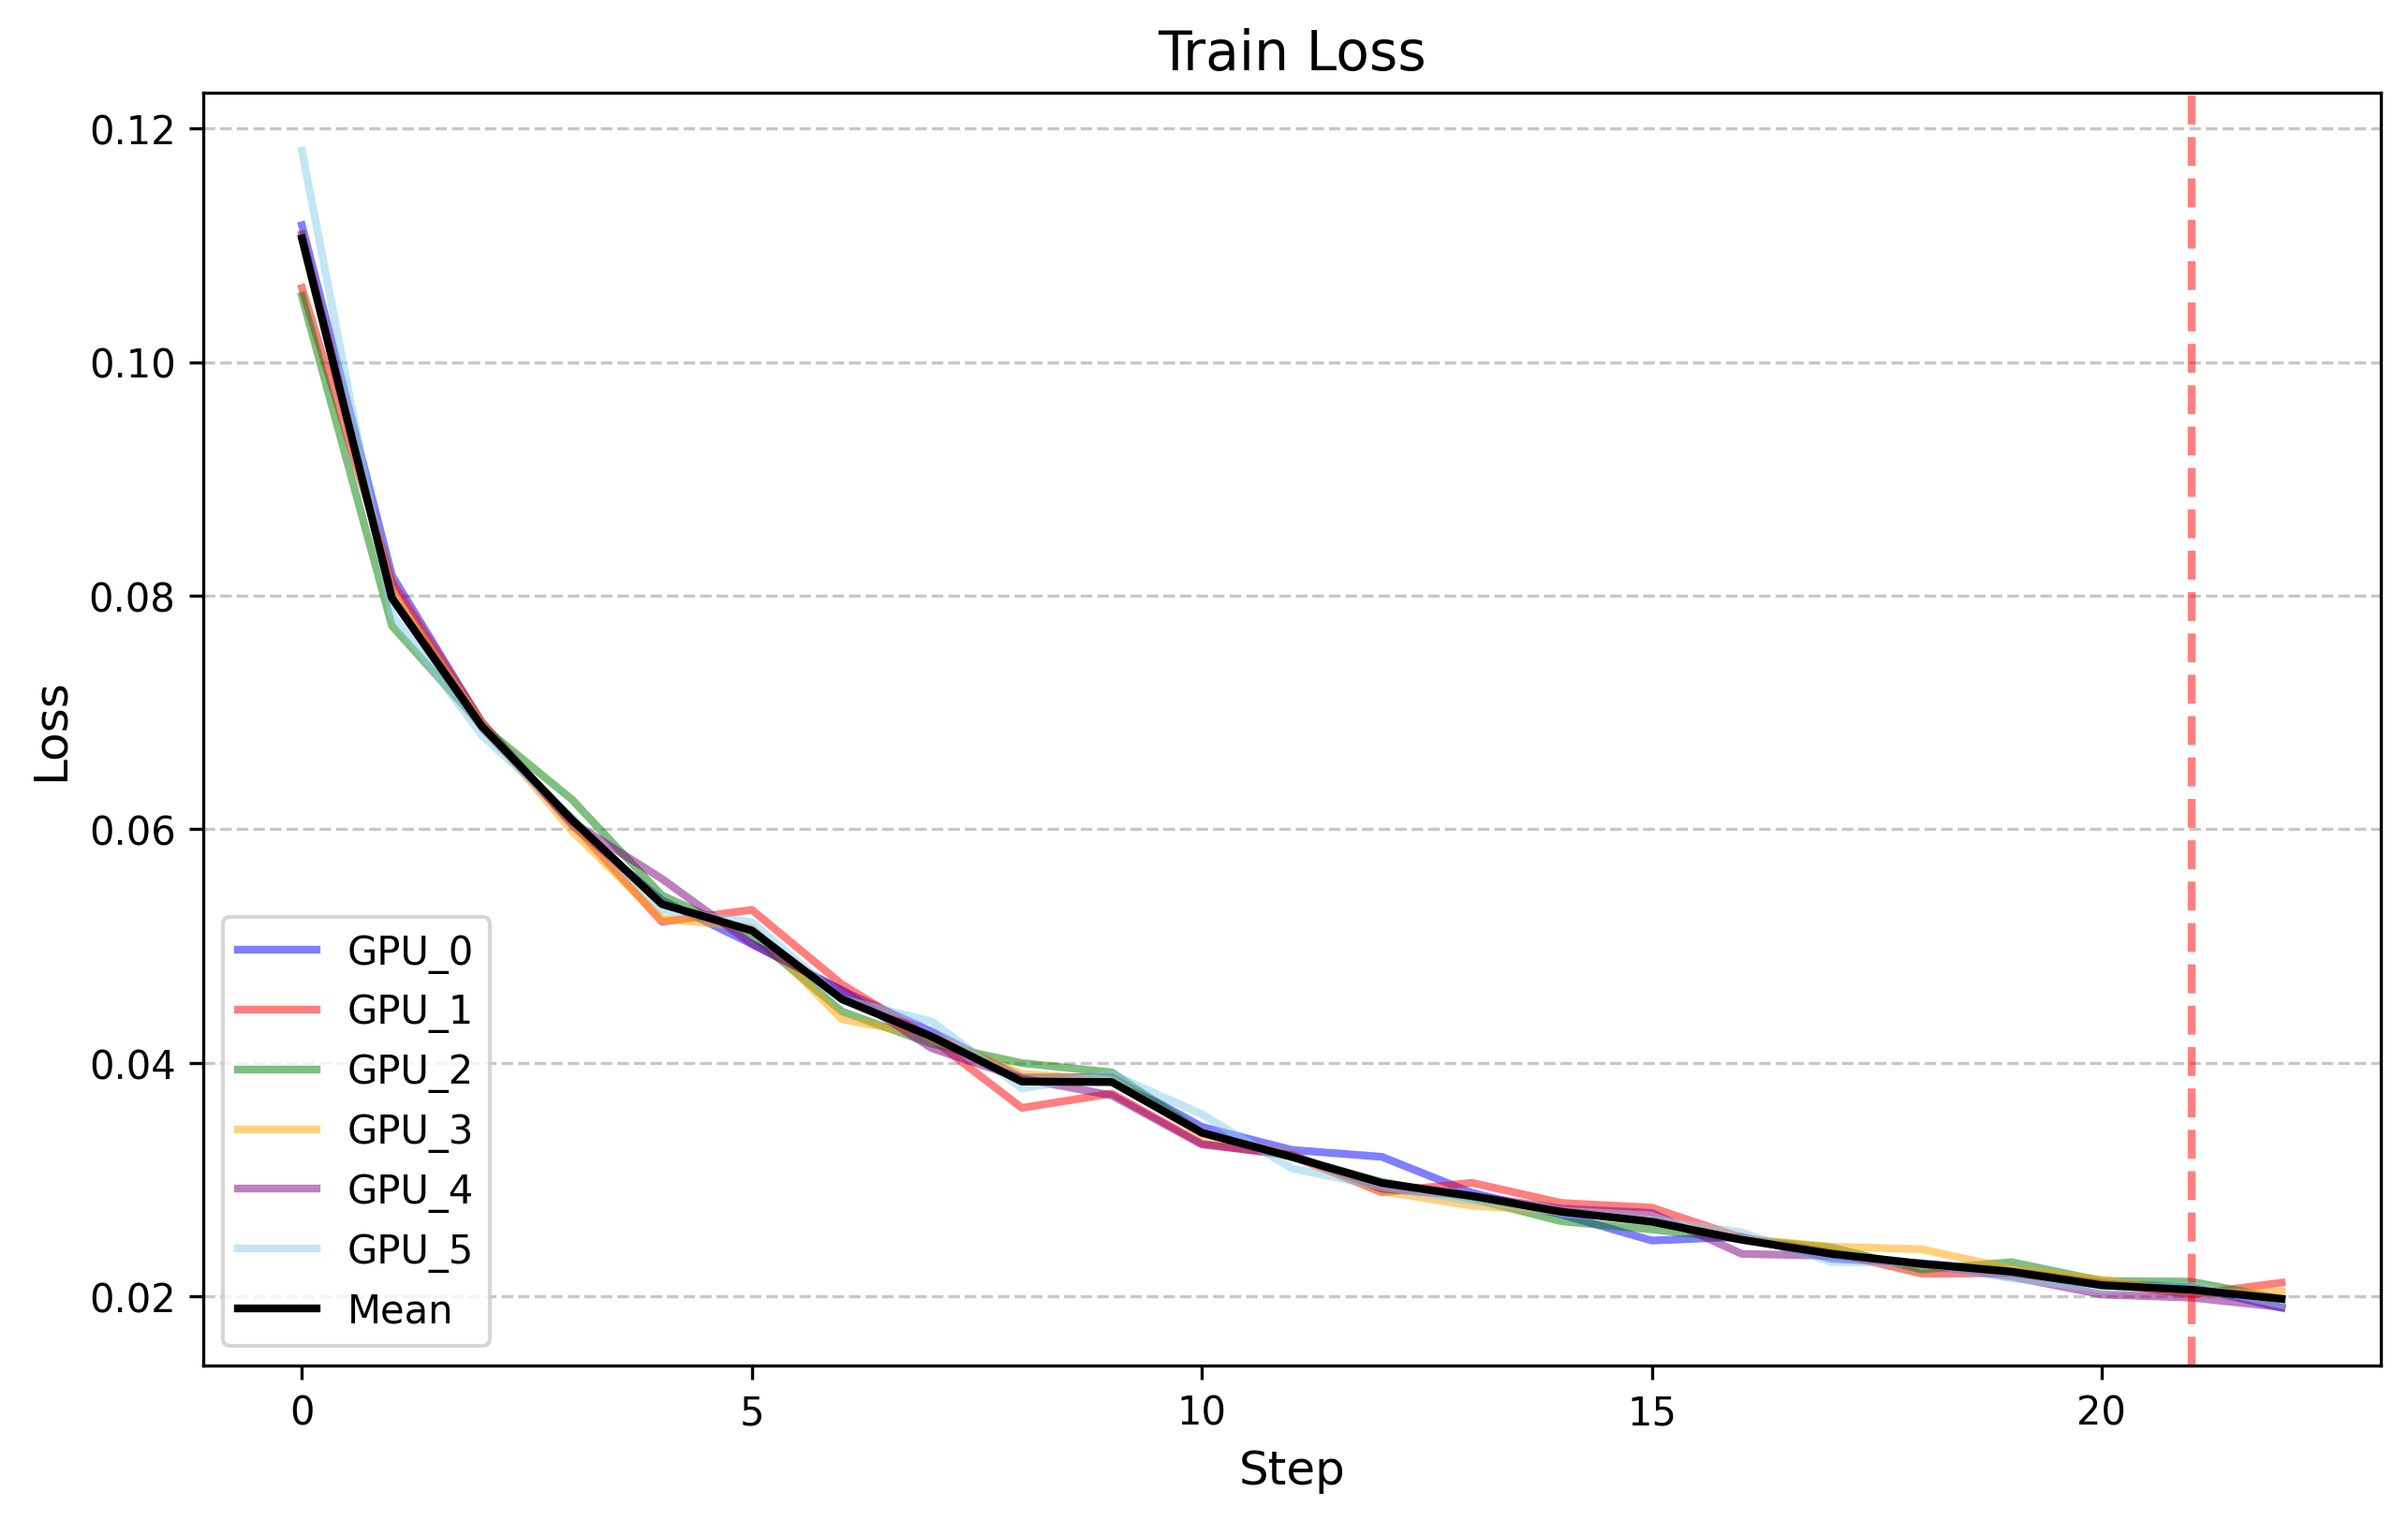
\includegraphics[width=\textwidth]{"images/train_loss.png"}
	\caption[Train loss \texttt{MyoSAM}]{Progression of \texttt{MyoSAM} train loss.}
	\label{figtrainloss}
\end{figure}
\begin{figure}[H]
	\centering
	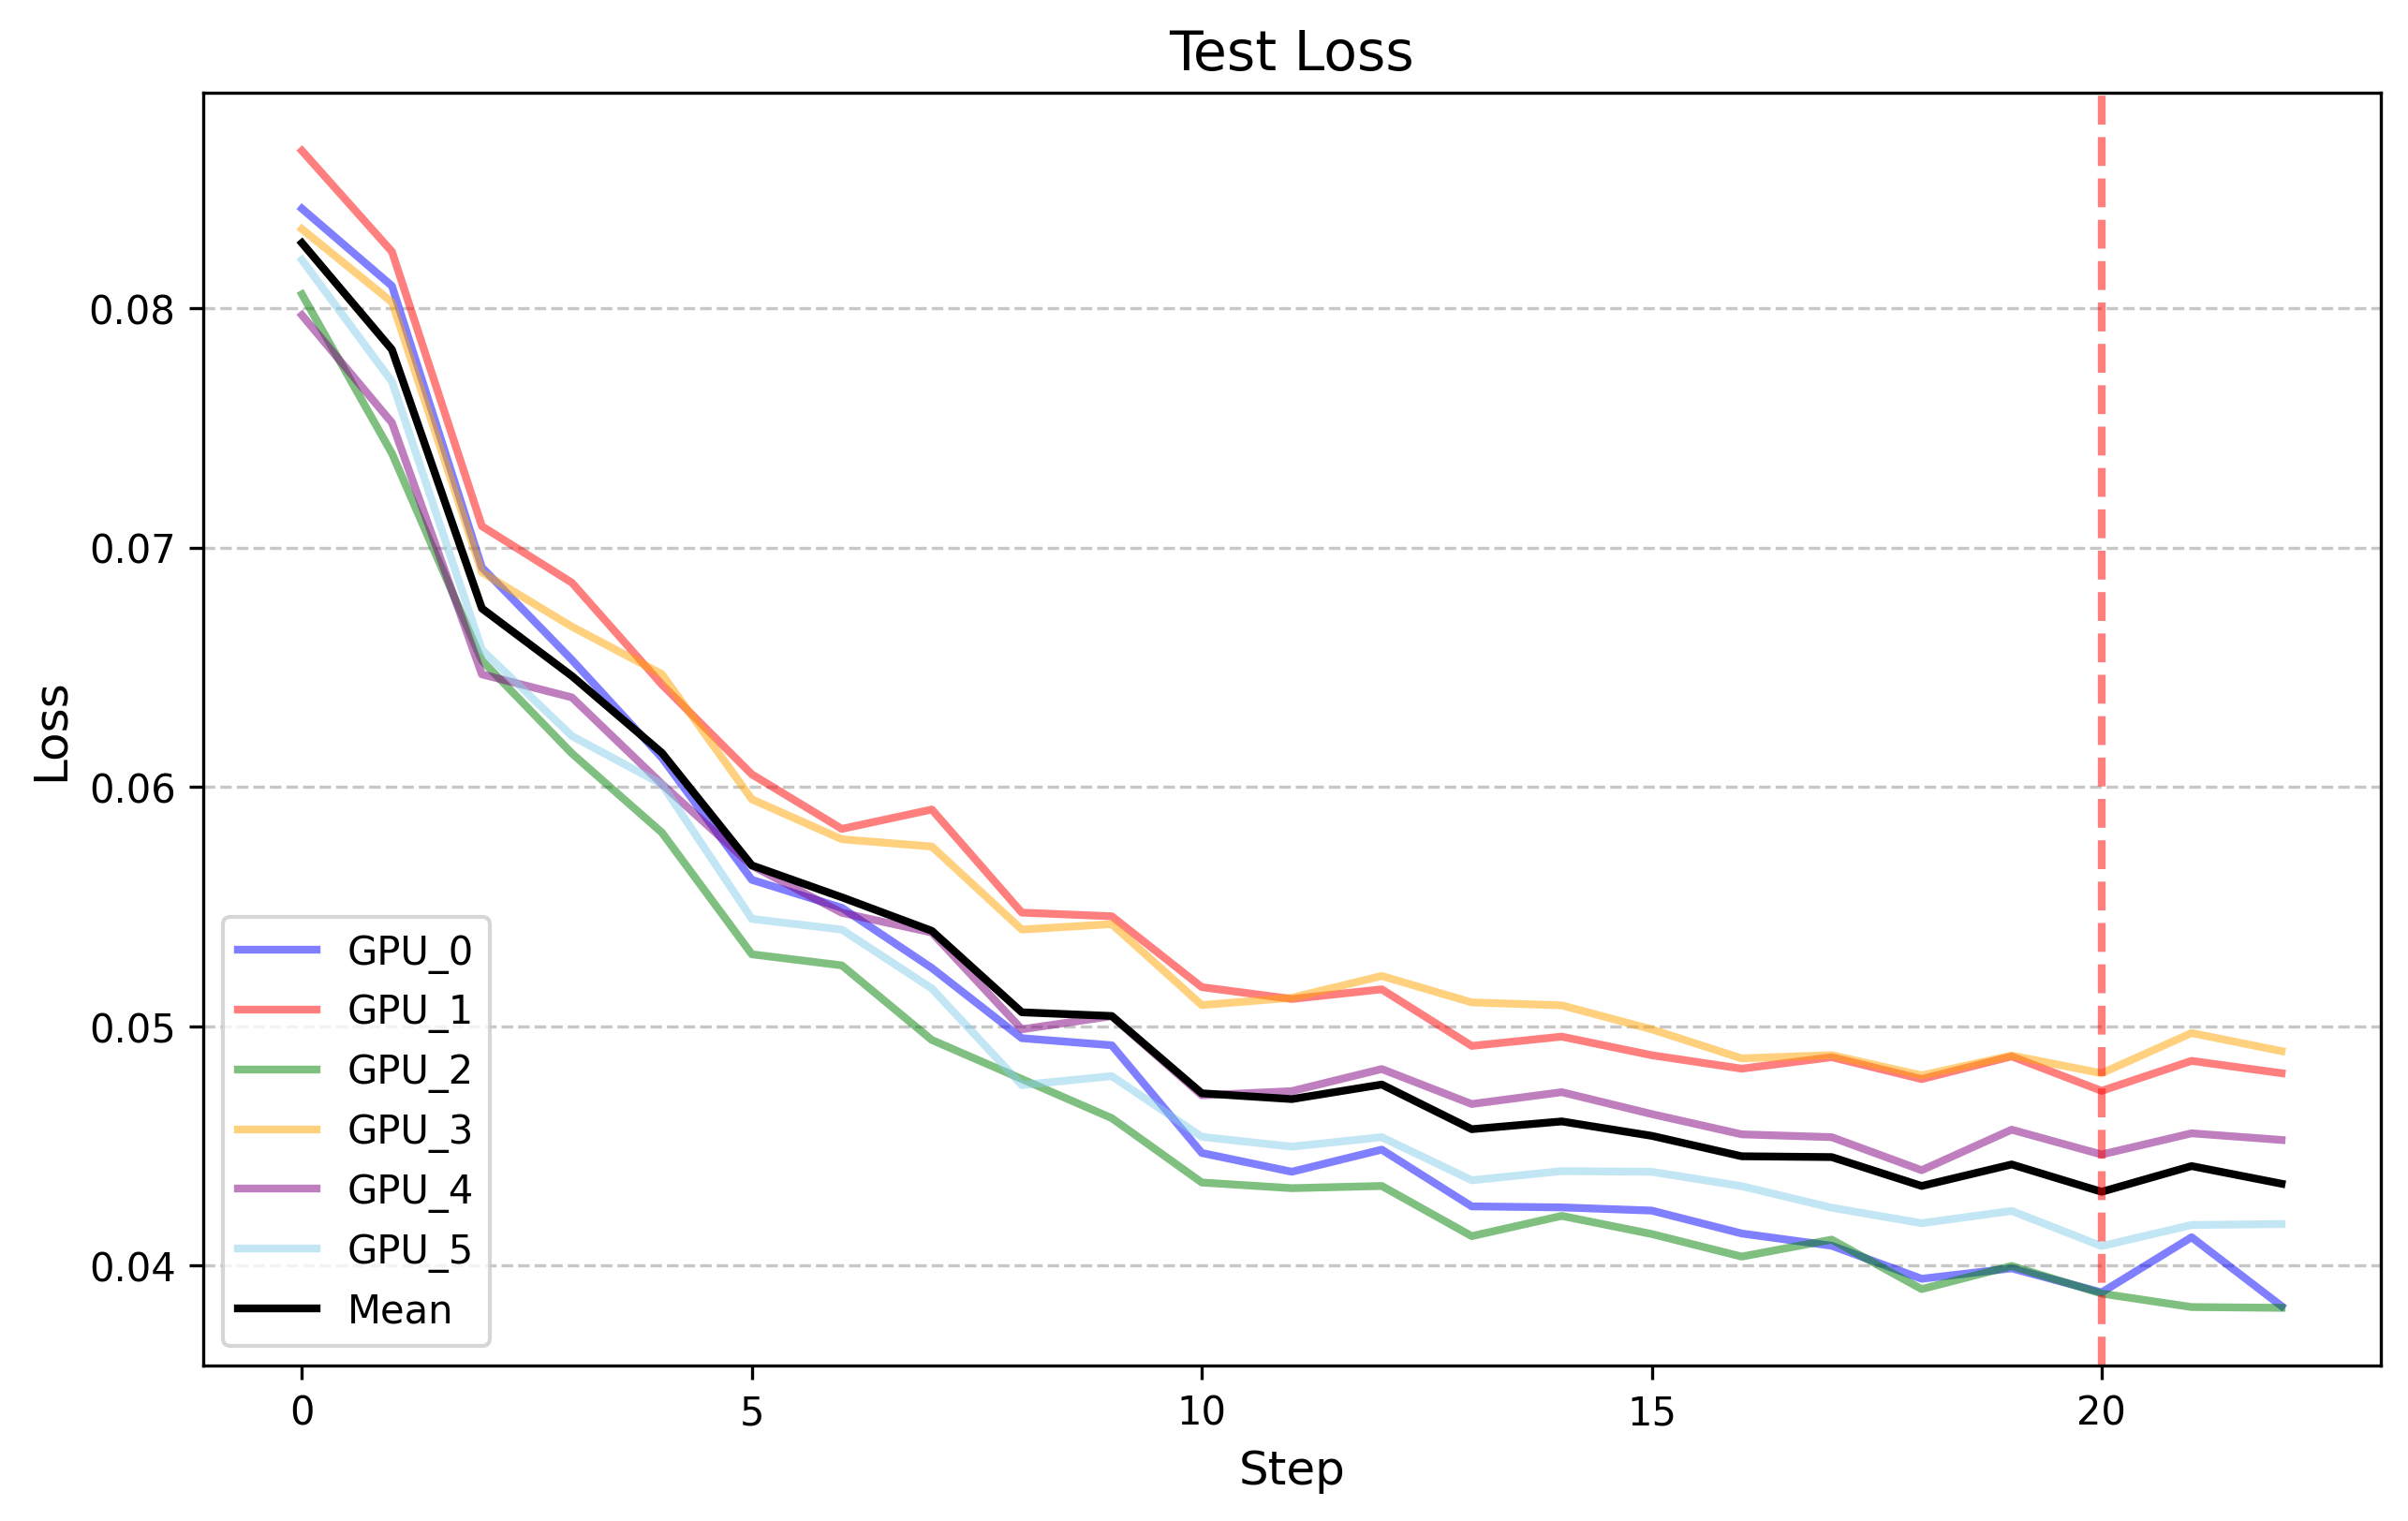
\includegraphics[width=\textwidth]{"images/test_loss.png"}
	\caption[Test loss \texttt{MyoSAM}]{Progression of \texttt{MyoSAM} test loss.}
	\label{figtestloss}
\end{figure}
\begin{figure}
	\centering
	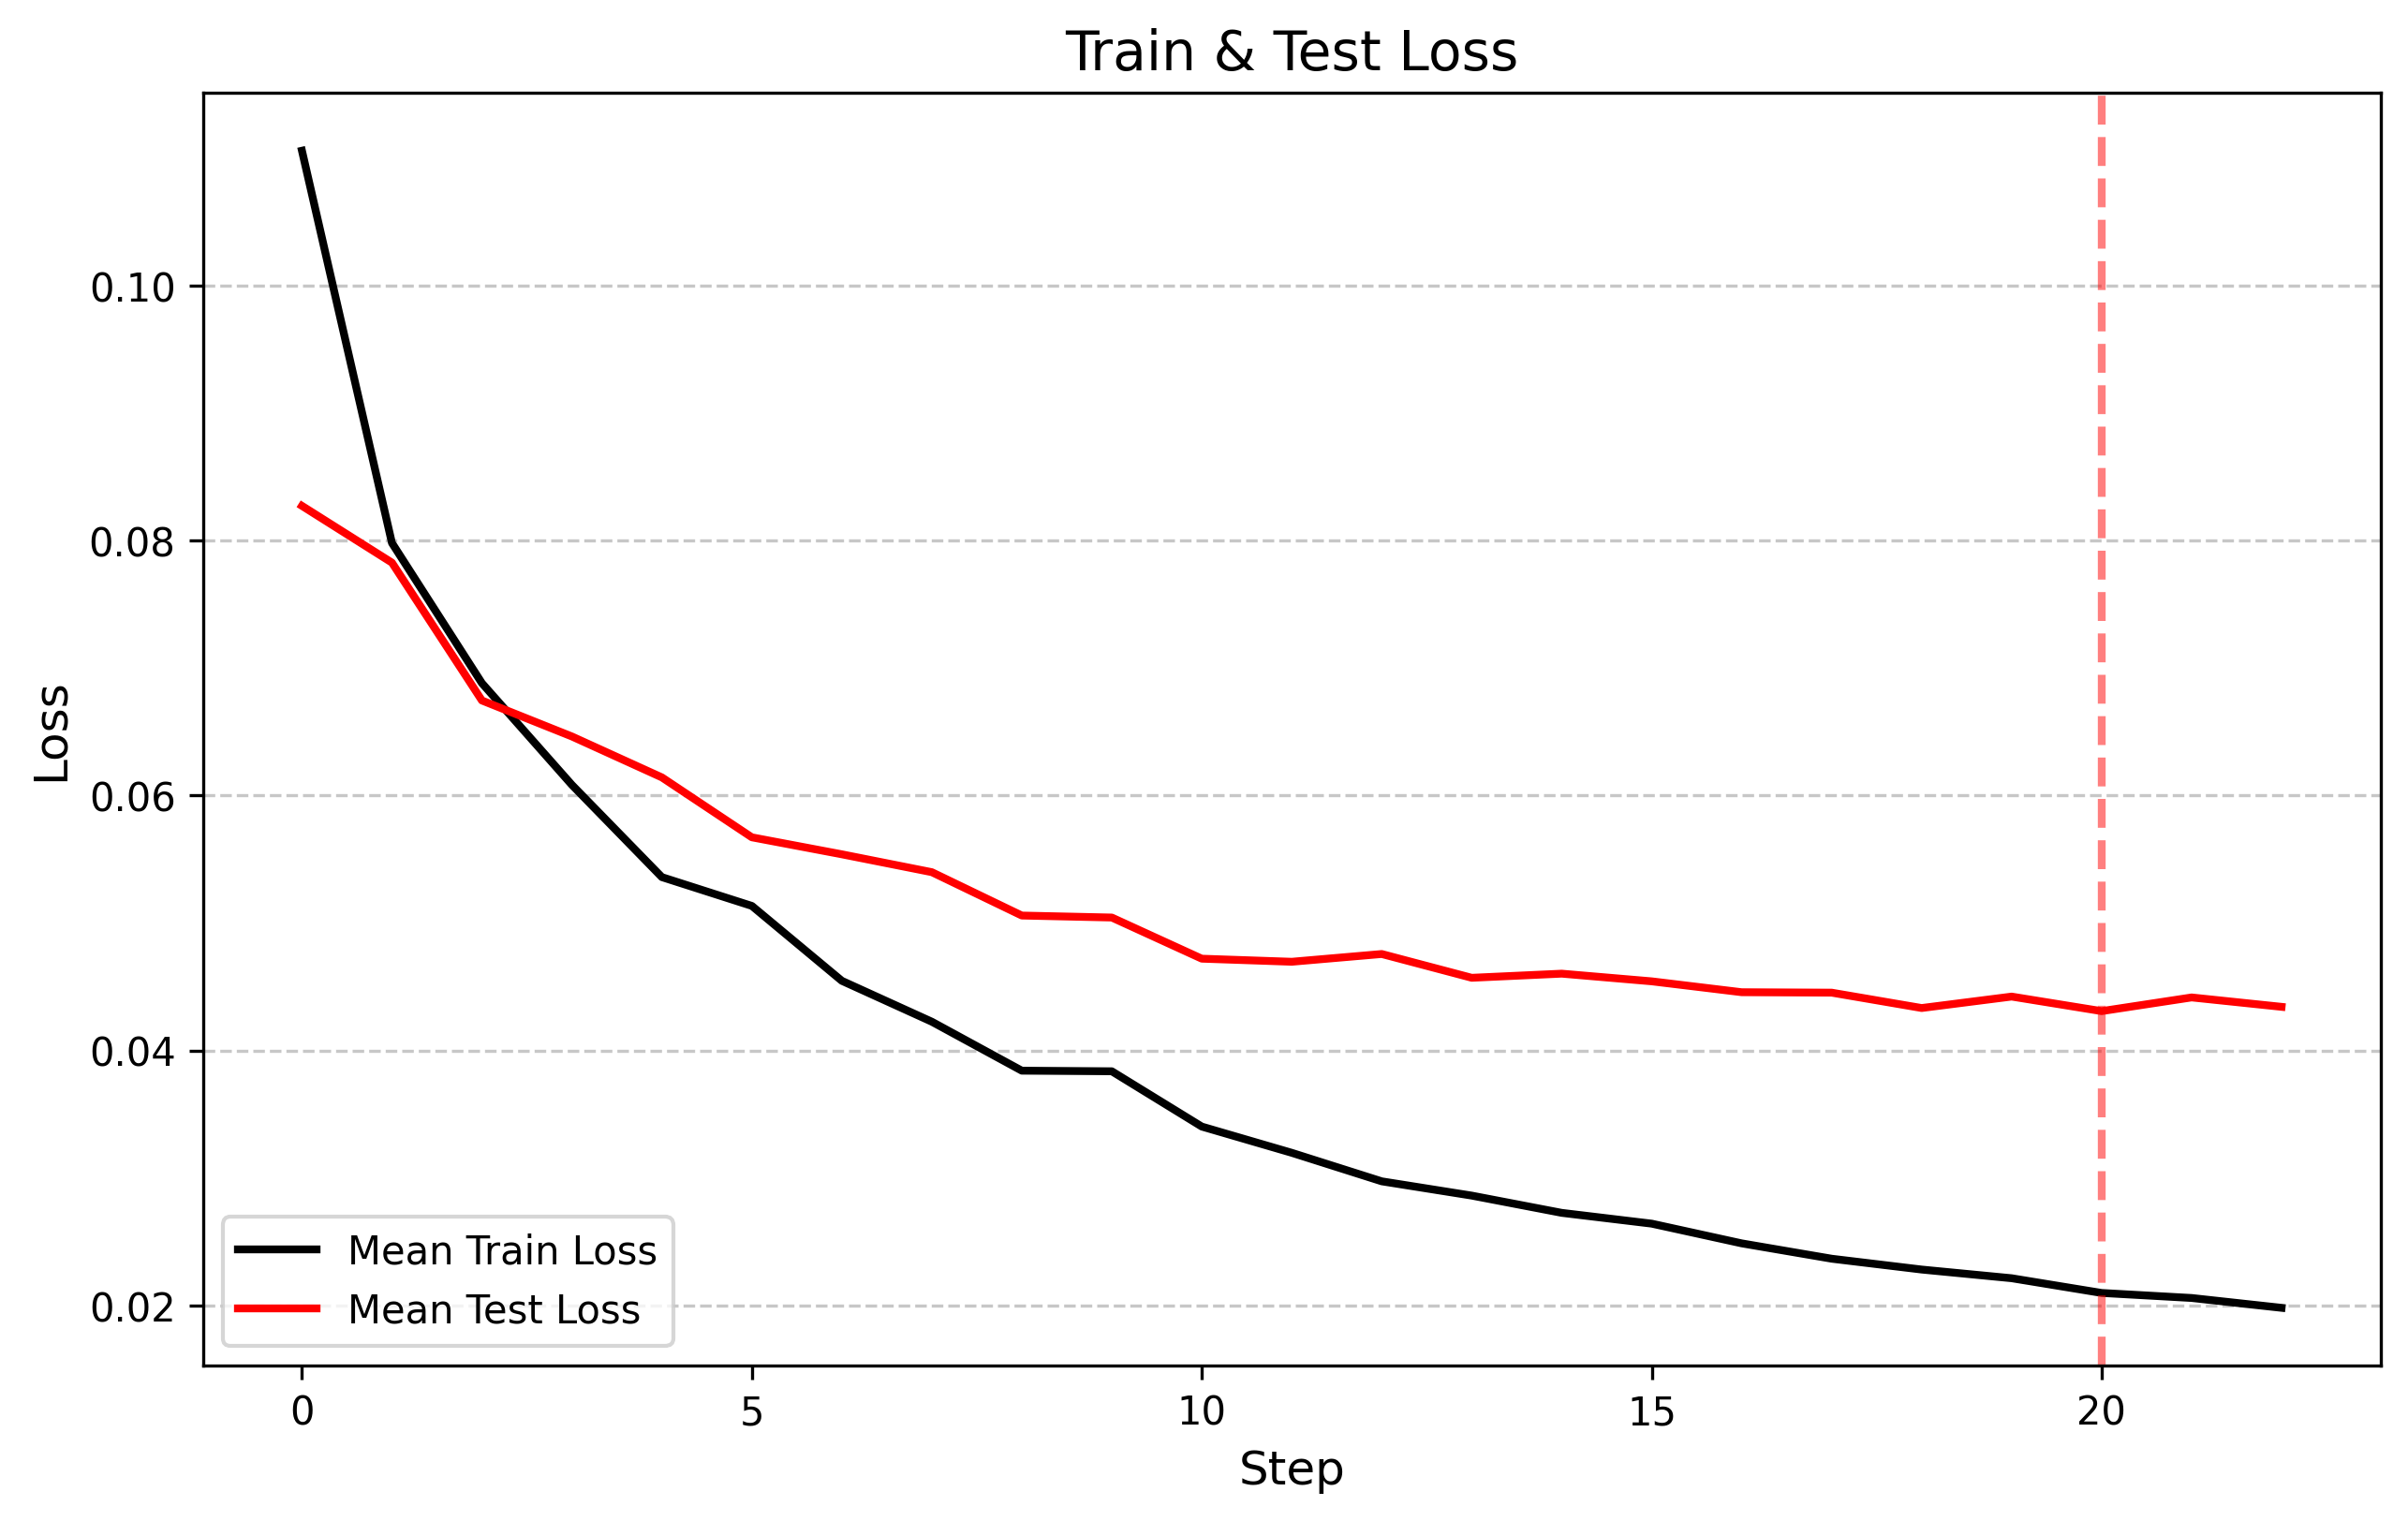
\includegraphics[width=\textwidth]{"images/train_test_loss.png"}
	\caption[Train and Test loss \texttt{MyoSAM}]{Comparison of \texttt{MyoSAM} loss progression.}
	\label{figtraintestloss}
\end{figure}
\subsection{Metrics}\label{secmetrics}
% Table 1: Image Specific Metrics
\begin{table}[H]
	\centering
	\label{tabimgspec}
	\caption{Image Specific Metrics}
	\begin{tabular}{|l|c|}
		\hline
		Metric & Formula \\
		\hline
		Total myotubes &  \\
		\hline
		Total nuclei &  \\
		\hline
		Total myoblasts &  \\
		\hline
		Total nuclei inside myotubes &  \\
		\hline
		Total fusion index & Total Fusion Index = $\frac{\text{N Nuclei in Myotubes}}{\text{N Nuclei}}$ \\
		\hline
		Number of nuclei clusters &  \\
		\hline
		Total myotube area &  \\
		\hline
		Total nuclei area &  \\
		\hline
		Total myoblasts area &  \\
		\hline
		Total nuclei inside myotubes area &  \\
		\hline
	\end{tabular}
\end{table}

% Table 2: Myotube Specific Metrics
\begin{table}[H]
	\centering
	\label{tabmyospec}
	\caption{Myotube Specific Metrics}
	\begin{tabular}{|l|c|}
		\hline
		Metric & Formula \\
		\hline
		Predicted IoU & IoU = $\frac{\text{Area of Overlap}}{\text{Area of Union}}$ \\
		\hline
		Stability &  \\
		\hline
		Is on edge &  \\
		\hline
		RGB min &  \\
		\hline
		RGB max &  \\
		\hline
		RGB mean &  \\
		\hline
		RGB median &  \\
		\hline
		RGB mode &  \\
		\hline
		RGB standard deviation &  \\
		\hline
		Integrated density RGB &  \\
		\hline
		Area &  \\
		\hline
		Convex area &  \\
		\hline
		Solidity & Solidity = $\frac{\text{Area}}{\text{Convex Area}}$ \\
		\hline
		Aspect ratio &  \\
		\hline
		Roundness & Roundness = $\frac{4 \times \text{Area}}{\pi \times \text{Major Axis}^2}$ \\
		\hline
		Perimeter &  \\
		\hline
		Feret’s Diameter (min \& max) &  \\
		\hline
		Circularity & Circularity = $\frac{4 \pi \times \text{Area}}{\text{Perimeter}^2}$ \\
		\hline
		Instance fusion index &  \\
		\hline
		Centroid &  \\
		\hline
		Cluster information &  \\
		\hline
	\end{tabular}
\end{table}

\begin{table}[H]
	\centering
	\caption{Performance Metrics and Their Corresponding Formulas}
	\label{tabdefs}
	\renewcommand{\arraystretch}{2}
	\begin{tabular}{|l|l|}
		\hline
		\textbf{Performance Metric} & \textbf{Formula} \\
		\hline
		Precision & $Precision = \frac{TP}{TP + FP}$ \\
		\hline
		Recall & $Recall = \frac{TP}{TP + FN}$ \\
		\hline
		Accuracy & $Accuracy = \frac{TP}{TP + FP + FN}$ \\
		\hline
		
		Intersection over Union (IoU) & $IoU(R,P) = \frac{|R \cap P|}{|R \cup P|}$ \\
		\hline
		
		Intersection over Reference (IoR) & $IoR(R,P) = \frac{|R \cap P|}{|R|}$ \\
		\hline
		
		Normalized Surface Distance (NSD) & $NSD(R,P)^{(\tau_{\text{NSD}})} = \frac{|S_R \cap B_P^{(\tau_{\text{NSD}})}| + |S_P \cap B_R^{(\tau_{\text{NSD}})}|}{|S_R| + |S_P|}$
		\\
		\hline
		Panoptic Quality (PG) & PQ = $\frac{\sum_{(R, P) \in TP} IoU(R, P)}{|TP| + \frac{1}{2}|FP| + \frac{1}{2}|FN|}$ \\
		\hline
	\end{tabular}\\	
\end{table}
Explanation of variables:
\begin{enumerate}
	\item $R$: Reference
	\item $P$: Prediction
	\item $S_R$: Boundary of $R$
	\item $B_R$: Border Regions of $R$
	\item $S_P$: Boundary of $P$
	\item $B_P$: Border Regions of $P$
\end{enumerate}
